\documentclass[a4paper,UTF8]{article}
\usepackage{ctex}
\usepackage[margin=1.25in]{geometry}
\usepackage{color}
\usepackage{graphicx}
\usepackage{amssymb}
\usepackage{amsmath}
\usepackage{amsthm}
\usepackage{enumerate}
\usepackage{bm}
\usepackage{hyperref}
\usepackage{minted}
\usepackage{pgf, tikz}
\usetikzlibrary{arrows}
\numberwithin{equation}{section}
%\usepackage[thmmarks, amsmath, thref]{ntheorem}
\theoremstyle{definition}
\newtheorem*{solution}{Solution}
\newtheorem*{prove}{Proof}
\newcommand{\indep}{\rotatebox[origin=c]{90}{$\models$}}

\usepackage{multirow}

%--

%--
\begin{document}
\title{机器学习导论\\
习题五}
\author{151250104, 卢以宁,  kiwiloveskiwis@gmail.com}
\maketitle
\section{[25pts] Bayes Optimal Classifier}
试证明在二分类问题中,但两类数据同先验、满足高斯分布且协方差相等时,LDA可产生贝叶斯最优分类器。
\begin{solution}
由题意, $p(c=0) = p(c=1), p(\mathbf{x}|c=0) = N(\mathbf{\mu_1}, \Sigma), p(\mathbf{x}|c=1) = N(\mathbf{\mu_2}, \Sigma)$ \\
则贝叶斯最佳判别面为: 
\begin{equation}
\begin{split}
p(c = 0| \mathbf{x})  &= p(c = 1 | \mathbf{x})  \\
\ln[p(c = 0) p(\mathbf{x}|c=0)] &=\ln[ p(c = 1)p(\mathbf{x}|c=1) ] \\
\mathbf{(x-\mu_1)^T} \Sigma^{-1} \mathbf{(x-\mu_1)} &= \mathbf{(x-\mu_2)}^T\Sigma^{-1} \mathbf{(x-\mu_2)} \\
\Sigma^{-1}\mathbf{(\mu_1-\mu_2)x} &= \frac{1}{2}  (\mu_1^T \Sigma^{-1} \mu_1 -  \mu_2^T \Sigma^{-1} \mu_2) %%%%%
\end{split}
\end{equation}
令$\mathbf{w}$为$\Sigma^{-1}\mathbf{(\mu_1-\mu_2)}$, $b$为$-\frac{1}{2}  (\mu_1^T \Sigma^{-1} \mu_1 -  \mu_2^T \Sigma^{-1} \mu_2)$即可。接下来证明使用 LDA 将得到相同结果。
\begin{equation}
\begin{split}
\min_{\mathbf{w}} & \quad \mathbf{-w^TS_bw} \\
\text{s.t.} & \quad \mathbf{-w^TS_ww} = 1
\end{split}
\end{equation}
解得
\begin{equation}
\begin{split}
\mathbf{w} &= \mathbf{S^{-1}_w(\mu_0 - \mu_1)}  \\
&= \sum_{x \in {X_0}} \mathbf{(x - \mu_0)(x - \mu_0)^T} + \sum_{x \in {X_1}} \mathbf{(x - \mu_1)(x - \mu_1)^T}\\
&= 2 \Sigma^{-1}\mathbf{(\mu_1-\mu_2)}
\end{split}
\end{equation}

则投影中心分别为$\mathbf{w\mu_0}$ 和 $\mathbf{w\mu_1}$. 故$b = -\frac{1}{2}(\mathbf{w\mu_0} + \mathbf{w\mu_1})$. 即 LDA 可以得到贝叶斯最优判别面。 

\end{solution}

\section{[25pts] Naive Bayes}
考虑下面的400个训练数据的数据统计情况,其中特征维度为2($\mathbf{x}=[x_1,x_2]$),每种特征取值0或1,类别标记$y\in\{-1,+1\}$。详细信息如表\ref{table:training}所示。

根据该数据统计情况,请分别利用直接查表的方式和朴素贝叶斯分类器给出$\mathbf{x}=[1,0]$的测试样本的类别预测,并写出具体的推导过程。
\begin{table}[h]
\centering
\caption{数据统计信息}
\label{table:training}\vspace{2mm}
\begin{tabular}{cc|cc}\hline
$x_1$		&  $x_2$ 	&	$y=+1$	&	$y=-1$ 	\\ \hline
0		&  0 	&	90	&	10 \\
0		&  1 	&	90 	&	10 \\
1		&  0 	&	51 	&	49 \\
1		&  1 	&	40 	&	60 \\\hline
\end{tabular}
\end{table}

\begin{solution}
(1) 查表方式: \\
\begin{equation}
P(y=+1 | x = [1, 0]) = 0.51 
\end{equation}
故预测 $y=1$. \\ 

(2) 朴素贝叶斯: \\
\begin{equation}
P(y = 1) = \frac{271}{400}, P(y=-1) = \frac{129}{400}
\end{equation}
\begin{equation}
\begin{split}
P({x_1=0 |  y=1}) &=  \frac{180}{271}, P({x_1=0| y=-1}) =  \frac{20}{129} \\ 
P({x_1=1| y = 1}) &=  \frac{91}{271}, P({x_1 = 1| y=-1}) =  \frac{109}{129} \\
P({x_2=0| y=1}) &=  \frac{141}{271}, P({x_2=0| y=-1}) =  \frac{59}{129} \\
P({x_2=1| y=1}) &=  \frac{130}{271}, P({x_2=1| y=-1}) =  \frac{70}{129} \\
\end{split}
\end{equation}

\begin{equation}
\begin{split}
\frac{P{(y=+1|x_1=1,x_2=0)}}  { P(y=-1|x_1=1,x_2=0) } &= \frac{ P( y = +1) \times P(x_1 = 1 | y = +1) \times P(x_2 = 0 | y =+ 1) }{   P( y = -1) \times P(x_1 = 1 | y = -1) \times P(x_2 = 0 | y = -1)  }  \\
&= \frac{271\cdot91 \cdot 141}{400\cdot 271 \cdot 271} / \frac{129\cdot 109 \cdot 59}{400\cdot 129 \cdot 129} = \frac{165199}{1742801} < 1
\end{split}
\end{equation}
故预测$y=-1$.
\end{solution}

\section{\textbf{[25pts]} Bayesian Network}
贝叶斯网(Bayesian Network)是一种经典的概率图模型,请学习书本7.5节内容回答下面的问题:

(1) \textbf{[5pts]} 请画出下面的联合概率分布的分解式对应的贝叶斯网结构:
\begin{equation*}
\Pr(A, B, C, D, E, F) = \Pr(A)\Pr(B)\Pr(C)\Pr(D|A)\Pr(E|A)\Pr(F|B, D)\Pr(G|D, E)
\end{equation*}

(2) \textbf{[5pts]} 请写出图\ref{fig-DAG}中贝叶斯网结构的联合概率分布的分解表达式。
\begin{figure}[h]
\label{fig-DAG}
\centering
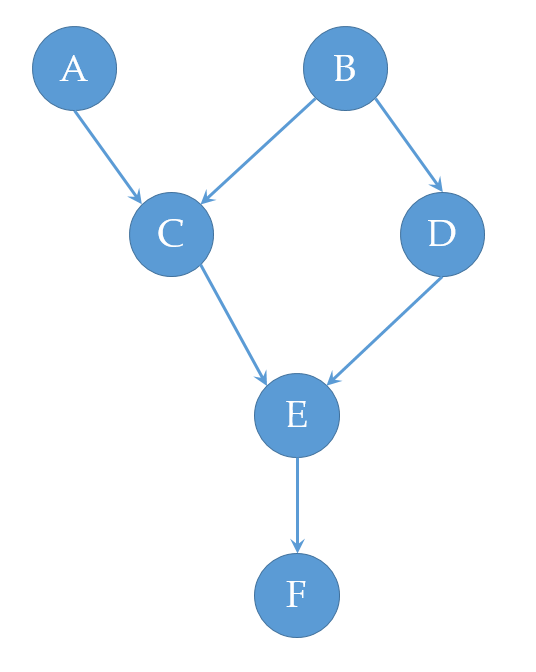
\includegraphics[scale=0.3]{bayes_net.png}
\caption{题目3-(2)有向图}
\end{figure}

(3) \textbf{[15pts]} 基于第(2)问中的图\ref{fig-DAG}, 请判断表格\ref{table:DAG}中的论断是否正确,只需将下面的表格填完整即可。
\begin{table}[h]
\centering
\caption{判断表格中的论断是否正确}
\label{table:DAG}
\begin{tabular}{c|l|c||c|l|c}\hline
序号   		& 		关系  		& True/False 	& 序号   	& 		关系  		& True/False \\ \hline
1			&	$A \indep B$ 		& 	True	    		& 7  		& 	$F \perp B|C$ 		& 	False		 \\
2			&	$A \perp B|C$ 	    	& 	False	    	& 8  		& 	$F \perp B|C, D$ 	& 	True		 \\
3			&	$C \indep D $		& 	False    		& 9  		& 	$F \perp B|E$ 		& 	True		 \\
4			&	$C \perp D|E$ 	& 	False	    	& 10  	& 	$A \indep F $		& 	False		 \\
5			&	$C \perp D|B, F$     	& 	False	    	& 11  	& 	$A \perp F|C$ 		& 	False		 \\
6			&	$F \indep B $		&  	False	    	& 12  	& 	$A \perp F|D$ 		& 	False		 \\ \hline
\end{tabular}
\end{table}

\begin{solution}
(1) \\
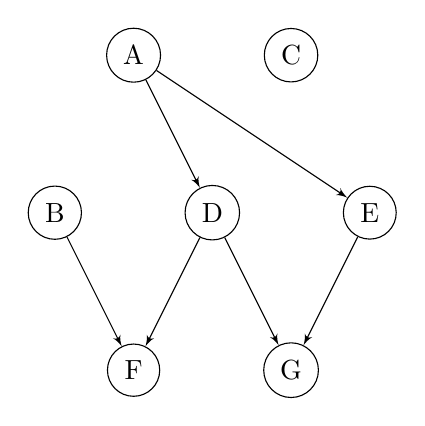
\begin{tikzpicture}
\tikzset{vertex/.style = {shape=circle,draw,minimum size=1.5em}}
\tikzset{edge/.style = {->,> = latex'}}
% vertices
\node[vertex] (a) at  (2,2) {A};
\node[vertex] (c) at  (4,2) {C};
\node[vertex] (b) at (1,0) {B};
\node[vertex] (d) at (3,0) {D};
\node[vertex] (e) at  (5,0) {E};
\node[vertex] (f) at  (2,-2) {F};
\node[vertex] (g) at  (4, -2) {G};
%edges
\draw[edge] (a) to (d);
\draw[edge] (a) to (e);
\draw[edge] (b) to (f);
\draw[edge] (d) to (f);
\draw[edge] (d) to (g);
\draw[edge] (e) to (g);
\end{tikzpicture} \\
(2) 
\begin{equation*}
\Pr(A, B, C, D, E, F) = \Pr(A)\Pr(B)\Pr(C|A, B)\Pr(D|B)\Pr(E|C, D)\Pr(F|E)
\end{equation*}

\end{solution}


\section{[25pts] Naive Bayes in Practice}
请实现朴素贝叶斯分类器,同时支持离散属性和连续属性。详细编程题指南请参见链接:\url{http://lamda.nju.edu.cn/ml2017/PS5/ML5_programming.html}. 

同时,请简要谈谈你的感想。实践过程中遇到了什么问题,你是如何解决的?
\begin{solution}
主要问题在于  对于数据集v0.0 不考虑连续变量时精度上升了将近一倍, 并且快了许多许多。我很想因此把连续变量忽略掉,但忍住了; 结论是tf-idf不适合用Naive Bayes. \\
但是更改后的数据集一劳永逸地解除了烦恼,(即使研究发现连续属性占了主导地位.) \\
至于连续属性有多举足轻重,我们进行了一个实验: 每次预测时, 从后 2500 维数据算出 
$\texttt{continuous\_prob\_sum}$
从前 2500 维数据算出 $\texttt{discrete\_prob\_sum}$ , 将它们的比例存下来. 
\begin{minted}{python}
RATIO = 1 # we don't know it yet

for ins in range(0, data.shape[0]):
	for cval in range(num_of_class): # class_value
		discrete_prob_sum = 0          
		continuous_prob_sum = 0  
		for i in range(0, 5000):
			if(i < 2500):
				discrete_prob_sum += ...
			else:
				continuous_prob_sum += ...
		ratio[ins, cval] = continuous_prob_sum / discrete_prob_sum	
		class_prob[cval] = np.log(cmat.shape[0] / data.shape[0]) 
	  		+ discrete_prob_sum + continuous_prob_sum * RATIO
	predict_y[ins] = np.argmax(class_prob)
.....
\end{minted}
得到ratio的结果如下(针对测试集): 
\begin{verbatim}
>>> np.mean(ratio, axis=0) 
array([ 2706665.65332563,  4083342.44150028,  4219538.94068223,
        3734542.59047444,  2785861.71508093])
>>> np.mean(ratio)
3505990.2682127017
\end{verbatim}
对于训练集: 
\begin{verbatim}
>>> np.mean(ratio, axis=0) 
array([ 2703279.99020332,  3436356.2750135 ,  3283160.81424551,
        3163941.63246489,  1676037.38363671])
>>> np.mean(ratio)
2852555.2191127865
\end{verbatim}
简单起见,我们使用了训练集全局的平均值2852555, 从而 $\texttt{RATIO = 1 / 2852555}$.在计算总 prob 时, 进行加权求和。 \\
注意到当我们仅使用离散属性进行预测时, 准确率为0.6639; 仅使用连续属性/两者皆使用进行预测时, 准确率为0.6844. 而在按上述方法预测时, 准确率达到0.7152. \\
真是要歌功颂德了呀。
~\\
~\\
~\\
\end{solution}
\end{document}